To perform the simulation,
first we create a list of calls to attend,
with time between calls,
according to the exponential distribution
with parameter indicated by each demand point.

We define two types of events, 
calls and releases, 
each time a call is attended,
generates a release,
that is inserted in the list of events, 
indicating that a server is busy.
If all servers are busy, the call is sent to queue.
\begin{figure}
  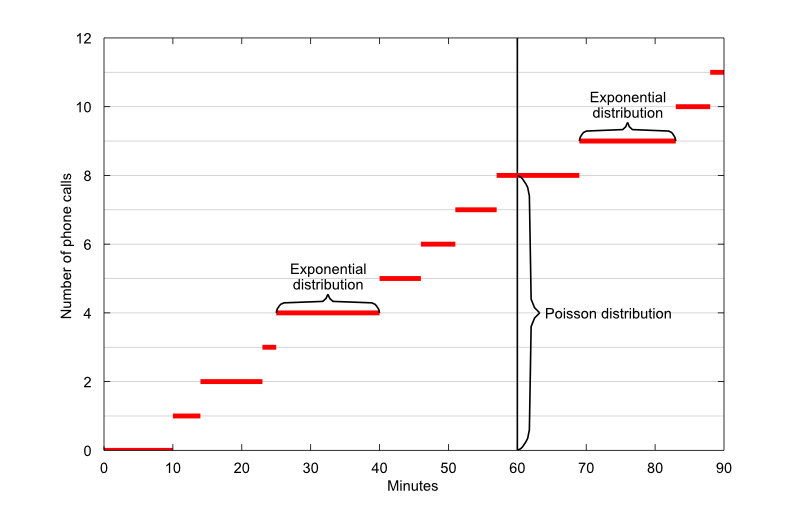
\includegraphics[width=7cm,keepaspectratio]{poisson_distribution}
\end{figure}
